\linespread{1.2}
\documentclass{beamer}
\usepackage{epstopdf}
\usepackage{tabularx}
\usepackage{amsmath}%
\usepackage{amscd} %allows drawing commutative diagrams
\usepackage{amsfonts}%
\usepackage{amssymb}%
\usepackage{graphicx}
\usepackage{color}

\newcommand{\noteLA}[1]{\textcolor{blue}{\footnotesize\textit{{noteLA: #1}}}} %this defines a new command for notes which has one argument
\def\noteLA #1{} %when activated, suppresses printing notes - remember to de-activate with %sign when sending draft text

\setbeamertemplate{navigation symbols}{}

%\usetheme{Rochester}
%\usetheme{Madrid}
\usetheme{Goettingen}
%\usetheme{Singapore}

\beamersetuncovermixins{\opaqueness<1>{25}}{\opaqueness<2->{15}}
\begin{document}
\title{Heterogeneity and the Distance Puzzle}  
\author[Archanskaia and Daudin]{Archanskaia E.\inst{*} and Daudin G.\inst{**}}
\institute{ \inst{*} KU Leuven
  \and
  \inst{**} PSL, LEDa, DIAL/SciencesPo, OFCE
}
\date{September 2019
%\today
\\
\vspace{.3cm}
%\textit{Congress of the European Economic Association, 2012}
} 
\begin{frame}[plain]
\titlepage
\end{frame}

%\section{Introduction} 
\begin{frame}[plain]\frametitle{Introduction}
\begin{itemize}
\vspace{0.3cm}
\item Is the world getting smaller?
\vspace{0.2cm}
\begin{itemize}
\item seems obvious to many observers of globalization ("Death of distance")
\item but conflicting evidence in gravity equations: trade has become more sensitive to distance since 1960s: Disdier  \&  Head, (2008), Head \& Mayer (2013)...
%meta-analysis by Disdier \& Head (2008)
\end{itemize}
\vspace{0.3cm}
\item What explains this `distance puzzle'?
\vspace{0.2cm}
\begin{itemize}
\item estimation strategy 
%(Santos Silva \& Tenreyro (2006), Bosquet \& Boulhol (2009))
\item composition effect \\
%(Berthelon \& Freund (2008), Duranton \& Storper (2008))
\noteLA{Contribute to but do not remove it}
\end{itemize}
\vspace{0.3cm}
\noteLA{Say here: world may be getting smaller while at the same time the elasticity of trade to distance may be non-decreasing. This is where ambiguity in distance puzzle appears.}
\item Not a puzzle, but a finding?
\vspace{0.2cm}
\begin{itemize}
\item relative growth in short vs. long-distance trade 
%(Buch et al. (2004))
\item evolution of distance-related trade costs
\begin{enumerate}
\item transport costs relatively to price of traded goods
%(Hummels \& Schaur (2012), Feyrer (2009), Hummels (2007), Daudin(2003, 2005))
\item growing importance of certain trade cost components 
%(time barrier)
\end{enumerate}
%\item evolution relatively to non-distance related trade costs
%what matters is not level, but the elasticity; relative evolution distance and non-distance dependent trade costs: loading cost at ports vs. fuel
%(Hummels \& Schaur (2012), Feyrer (2009), Hummels (2007), Daudin(2003, 2005))
\vspace{0.3cm}
\end{itemize}
\end{itemize}
\end{frame}

\begin{frame}[plain]\frametitle{Motivation}
\vspace{0.3cm}
\begin{itemize}
\item The contribution:
\vspace{0.2cm}
\begin{itemize}
\item take microfoundations of the gravity equation seriously
\item to provide a direct explanation of the increasing distance elasticity of trade over long time period
%1963-2009
\end{itemize}
\vspace{0.3cm}
\item The trick? 
\vspace{0.2cm}
\begin{itemize}
\item distance coefficient is a product of two elasticities:
\begin{enumerate}
\item elasticity of trade to trade costs (`heterogeneity')
%this is our focus: heterogeneity parameter: this parameter could have increased precisely because the world is shrinking...will come back to this in part 2 of the talk; this is the important economic parameter: Arkolakis et al.: crucial parameter for welfare computations across models
\item elasticity of trade costs to distance (`pop debate')
%this is the parameter the pop debate is centered on: this is where `puzzle' comes from: idea that increasing elasticity of trade costs to distance would be somewhat puzzling in a world where we may think that advances in transport and communications technology have reduced the \%-increase in trade costs to a 1\% increase in bilateral distance
\end{enumerate}
\item focus on the parameter capturing heterogeneity
%the trade elasticity ($\sigma$, $\theta$, $\gamma$)
\item to refine understanding of how the world is shrinking 
\vspace{0.3cm}
%to document what is driving the distance puzzle
%pop debate puzzle `solved': an increase in the elasticity of trade costs to distance could be puzzling, but there is no such thing in the data 
\end{itemize}
\vspace{0.3cm}
\item The message?
\begin{itemize}
\item Not only... reduction in trade cost elasticity to distance
\item But also... increasing similarity of countries \\
\hspace{1.5cm} in a model-specific dimension
%Evolution of heterogeneity parameter provides a direct explanation of the distance puzzle 
%reinforced shrinking: not only world getting less sensitive to distance, but also world becoming more similar. In our case: in terms of exporter-bundles.
\end{itemize}
\end{itemize}
\end{frame}

\begin{frame}[plain]\frametitle{Summary of results}
\vspace{0.3cm}
\begin{itemize}
\item Robustness of distance puzzle in 1962-2009: increase in distance coefficient 
%Working with COMTRADE bilateral trade data at the 4-digit level 
\begin{itemize}
\item 7\% controlling for estimation strategy
\item 14\% controlling for composition and sample effects
\end{itemize}
\vspace{0.3cm}
\item Evolution of heterogeneity parameter:
\begin{itemize}
\item 13\% increase in 1963-2009 (19\% in 1970-2009)
\item this estimate is likely to be a lower bound 
\end{itemize}
\vspace{0.3cm}
\item Elasticity of trade costs to distance has not increased
\begin{itemize}
\item 5-7\% decrease in 1963-2009
%depending on whether we work with evolution of ratio or with ratio of trends 
\item 17\% decrease in 1970-2009 
%in our data: the increase in the distance elasticity mainly driven by 62-70 period; since 70s distance elasticity flat
%this is also caveat of what we do: magnitude of results (their statistical robustness) is period-sensitive, but the direction of the change is robust to the time period
\end{itemize}
\vspace{0.3cm}
\item Which dimension of increased country similarity? 
\begin{itemize}
\item Result obtained within the Armington framework 
\vspace{0.3cm}
\item Increased substitutability of traded product bundles 
%Reduced heterogeneity means increased substitutability of exporter-specific product bundles
\end{itemize}
\end{itemize}
\end{frame}
%motivation of presenting results for 1970-2009: period in which air transportation has become an important transport means in trade
%message in one sentence: evolution of heterogeneity parameter provides direct explanation of increase distance elasticity of trade while composition and sample effects deepen the distance puzzle (composition: consistent with increasing share of manuf goods in trade (commodities and reference priced goods are more substitutable); sample: consistent with idea that countries which are stable trade partners may have witnessed relatively more similarity of export bundles than if all changes in sample of trading pairs allowed). Notice that cumulated effect composition and sample still at +14\% which means that stable partners are maybe also those which have experienced less changes in terms of composition of traded goods (manuf already in 62, and therefore no additional kick from composition effects). Thus, our analysis of composition and sample effects does tell a convincing story about world trade patterns: for unstable partners, more heterogeneity in bundles but stronger increase in share of manuf overtime; for stable partners, less movement in share of manuf but more movement in terms of reduced heterogeneity of exchanged varieties in manuf. 
%Not useful to say but say if questioned: For this parameter to be true trade elasticity across models would correspond to a very strong assumption on fixed trade costs: so small that all firms enter all export markets, and therefore only intensive margin matters.
%think about Egger argument about home bias: mechanical increase in distance sensitivity of trade flows as countries grow?

\begin{frame}[plain]\frametitle{Roadmap}\tableofcontents
\end{frame} 
%Say: I will go quickly over documenting the presence of distance puzzle in our data b/c this finding is present in several papers. The objective is to have sufficient time to explain our estimation methodology and results on the evolution of the heterogeneity parameter.

\section{The distance puzzle in our data}
\subsection{Benchmark estimation}
\begin{frame}\frametitle{Estimation procedure (1)}
\begin{itemize}
\item Microfounded gravity equation:
\begin{eqnarray}
X_{ij,t} & = & \left(\frac{Y_{i,t}Y_{j,t}}{Y_t}\right)\left(\frac{\tau_{ij,t}}{\Pi_{i,t}P_{j,t}}\right)^{-\zeta_t} \nonumber
\end{eqnarray}
%where the above formula is the standard gravity equation which can be derived across frameworks
\item heterogeneity parameter: $\zeta_t$: $\sigma_{t}-1$ in Armington 
\vspace{.3cm}
%$X_{ij,t}$ is the value of goods from country $i$ consumed in country $j$ in year $t$, i.e. bilateral imports at cif prices. Imports are a function of the nominal income of each trading partner $Y_{ij,t}$ and $Y_{j,t}$, of world income $Y_t$, of bilateral trade costs $\tau_{ij,t}$, and of inward and outward multilateral trade resistance terms $\Pi_{i,t}$, $P_{j,t}$.
\item Trade costs: 
\begin{itemize}
\item time-invariant cost controls (adjacency,...): $Z_1$
\item time-varying cost controls (policy: FTAs,...): $Z_2$
%potentially time-varying, therefore includes same country, colonial linkages, so on
\end{itemize}
\begin{gather}
\tau_{ij,t}=exp\left\{\rho_t\ln{dist_{ij}}+{Z_{1}}'\beta_{1,t}+{Z_{2,t}}'\beta_{2,t}\right\} \nonumber
\end{gather}
\item $\rho_t$ is the `world shrinkage' parameter \\ 
\hspace{1cm} i.e. elasticity of trade costs to distance
% (`shrinkage') 
%As is standard in the gravity literature, we model bilateral trade costs as a function of bilateral distance $dist_{ij}$, a vector $Z_1$ of bilateral trade cost controls such as adjacency, common language, colonial linkages, belonging or having once belonged to the same country, and a vector $Z_2$ of trade cost controls linked to trade policy such as common membership of GATT/WTO and common membership of an FTA. 
\end{itemize}
\end{frame}

\begin{frame}[plain]\frametitle{Estimation procedure (2)}
\begin{itemize}
\item COMTRADE data, 4-digit level (SITC), 1962-2009
%600-700 goods, little sensitivity to changes in classification: within-sitc rev.1 splits, seldom shuffling of goods across categories b/c all following revisions give more detail than initial sitc rev 1.
\vspace{.3cm}
\item run gravity equations (obviously)
\item cross section, no panel
\item focus on evolution of distance elasticity overtime
\vspace{.3cm}
\item using the PPML estimator (consistency \& efficiency)
%to deal with heteroskedasticity of trade equation in levels and to take into account zero flows
%Santos Silva and Tenreyro have shown that slope estimates from the log linear estimation of the gravity equation will generally be biased because the trade equation in levels is subject to heteroskedasticity. The structure of trade data is such that in general the additive error term in the log-linearized model is heteroscedastic, and its variance depends on the regressors. In this case, OLS does not generally give consistent slope estimates. PPML consistent and efficient: the mean and variance function this estimator assumes is closest to the underlying conditional variance function in raw trade data. The PPML is likely to be an efficient estimator because it assumes that the conditional variance of the raw data is proportional to the conditional mean. This fits trade data better than alternative assumptions on conditional variance of other non-linear estimators.
%Say: PPML implied functional form not consistent with the prevalence of zero trade observations (Vuong test), and therefore we have tested that results not sensitive to switching to a two-part approach where the proba of trading is estimated in the first step. The fact of the matter is that using ZIP does not change results conditional on trading but the implementation encounters convergence problems in certain years. Therefore, benchmark estimation in PPML while robustness check with two part approach which couples the PPML estimator with a logit estimation of the chances of being in the zero category.
\vspace{.3cm}
\item Estimated equation:
\begin{gather}
X_{ij,t}=\exp{\left(cons_t-\alpha_{t}\ln{dist_{ij}}+{Z_1}'\beta_{1,t}+{Z_{2,t}}'\beta_{2,t}+fe_{i,t}+fe_{j,t}\right)\epsilon_{ij,t}} \nonumber
\end{gather}
%multiplicative model
\item distance elasticity: $\alpha_{t}=\zeta_{t}\rho_t$
%exporter and importer dummies: $fe_{i,t}$, $fe_{j,t}$
\vspace{.3cm}
\item Baseline: trade policy controls excluded (FTAs)
\end{itemize}
\end{frame}

\begin{frame}[plain]\frametitle{Baseline regression (PPML)}
\begin{figure}[h!]
%\caption{Distance coefficient in the baseline PPML regression \label{fig:distcoefbaseline}}
\begin{center}
\setlength{\fboxrule}{1pt} %makes border lines thick
\setlength{\fboxsep}{.1in} %increases distance to border
\fbox{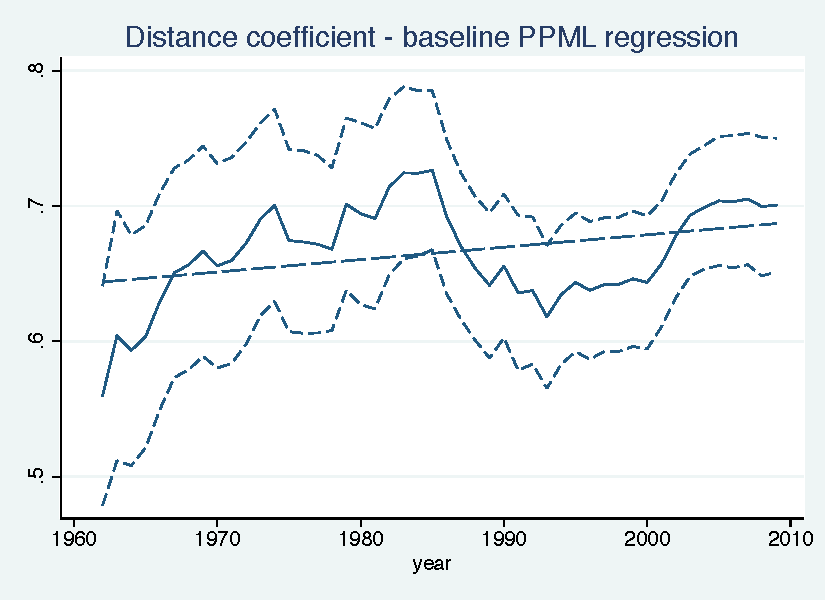
\includegraphics[trim = 0mm 0mm 0mm 9.5mm, clip, height=2.5in]{graph1.pdf}}
\end{center}
\end{figure}
%\vspace{0.3cm}
%8\% increase in distance elasticity
\end{frame}

\if 0
\begin{frame}[plain]\frametitle{Logit baseline ZIP regression}
\begin{figure}[h!]
%\caption{Distance coefficient in the logit baseline ZIP regression (first part)\label{fig:distcoefbaselinelogit}}
\begin{center}
\setlength{\fboxrule}{1pt} %makes border lines thick
\setlength{\fboxsep}{.1in} %increases distance to border
\fbox{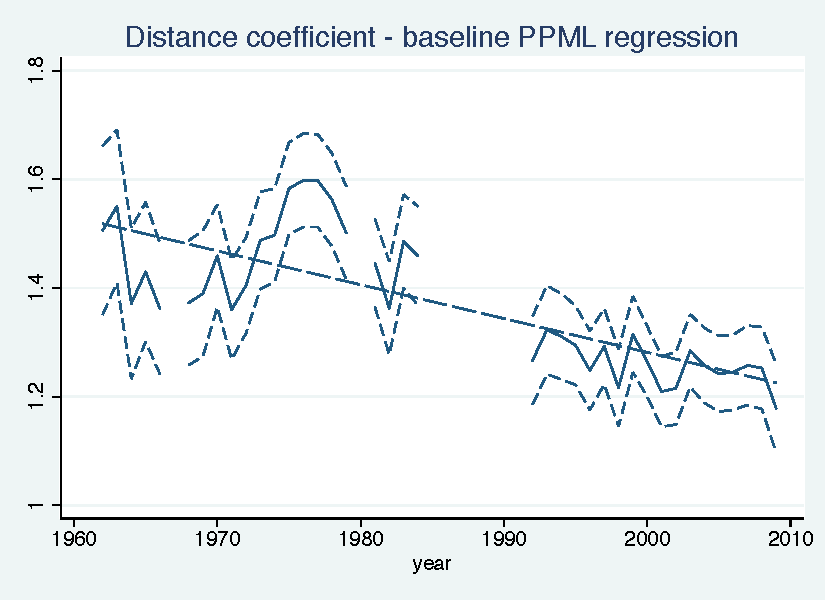
\includegraphics[trim = 0mm 0mm 0mm 9.5mm, clip,height=2.5in]{graph3.pdf}}
\end{center}
\end{figure}
%\vspace{0.3cm}
%circumscribe puzzle: formation of trading relationships is less sensitive to distance; distance puzzle specific to existing trade relationships
\end{frame}
\fi

\subsection{Composition, sample, FTA effects}
\begin{frame}\frametitle{Robustness of puzzle}
\vspace{0.3cm}
%Explore three issues:
\begin{itemize}
\item Sample
\begin{itemize}
\item Test: keep only trading pairs that have reciprocal non-zero trade every year from 1962 to 2009
%similar results if square: all with all in each year
\item It deepens the puzzle 
\end{itemize}
\vspace{0.3cm}
\item Composition
\begin{itemize}
\item Test: suppose the composition of trade constant i.e. at 1962 shares for 4 digit goods
\item It deepens the puzzle (increse in manuf share)
%The share of manufacture goods increases : these are less sensible to distance
\end{itemize}
\vspace{0.3cm}
%Remark: most short-term fluctuations of the distance coefficient seem to be explained by sample and composition effects.
\item FTAs
\begin{itemize}
\item Test: introduce FTA variables
\item It `solves' the puzzle
\item But what does it mean ? 
\item Increasing number of proximity controls overtime 
\item Mechanically reduces the effect of distance
\end{itemize}
\end{itemize}
\end{frame}
%interpretation of composition and sample effects.
%composition: consistent with increasing share of manuf goods in trade (commodities and reference priced goods are more substitutable); sample: consistent with idea that countries which are stable trade partners may have witnessed relatively more similarity of export bundles than if all changes in sample of trading pairs allowed). Notice that cumulated effect composition and sample still at +14\% which means that stable partners are maybe also those which have experienced less changes in terms of composition of traded goods (manuf already in 62, and therefore no additional kick from composition effects). Thus, our analysis of composition and sample effects does tell a convincing story about world trade patterns: for unstable partners, more heterogeneity in bundles but stronger increase in share of manuf overtime; for stable partners, less movement in share of manuf but more movement in terms of reduced heterogeneity of exchanged varieties in manuf. 
\begin{frame}[plain]\frametitle{Composition}
\begin{figure}[h!]
%\caption{Distance coefficient controlling for composition (1962 weights) \label{fig:comp}}
\begin{center}
\setlength{\fboxrule}{1pt} %makes border lines thick
\setlength{\fboxsep}{.1in} %increases distance to border
\fbox{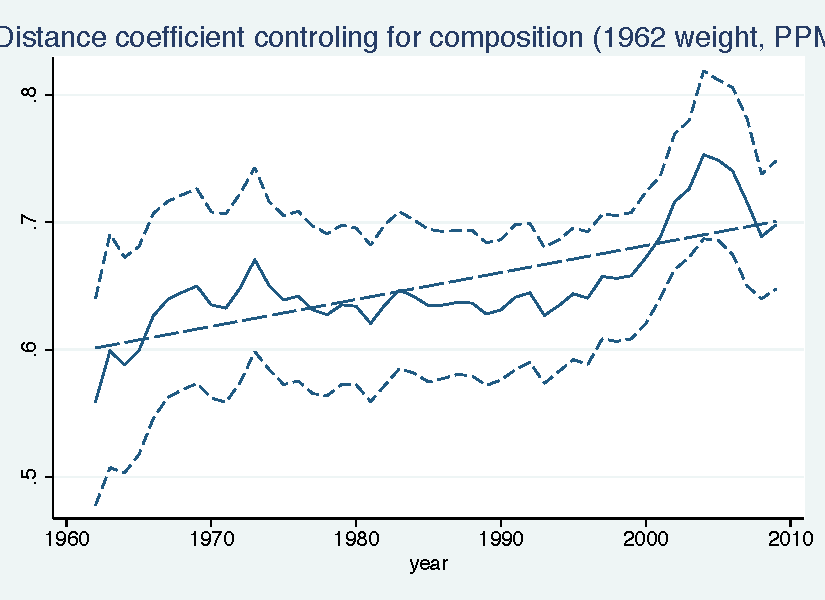
\includegraphics[trim = 0mm 0mm 0mm 9.5mm, clip,height=2.5in]{graph5.pdf}}
\end{center}
\end{figure}
\end{frame}

\if 0
\begin{frame}[plain]\frametitle{Sample}
\begin{figure}[h!]
%\caption{Distance coefficient in sample of stable pairs (PPML) \label{fig:distcoefbaselinesuperbal}}
\begin{center}
\setlength{\fboxrule}{1pt} %makes border lines thick
\setlength{\fboxsep}{.1in} %increases distance to border
\fbox{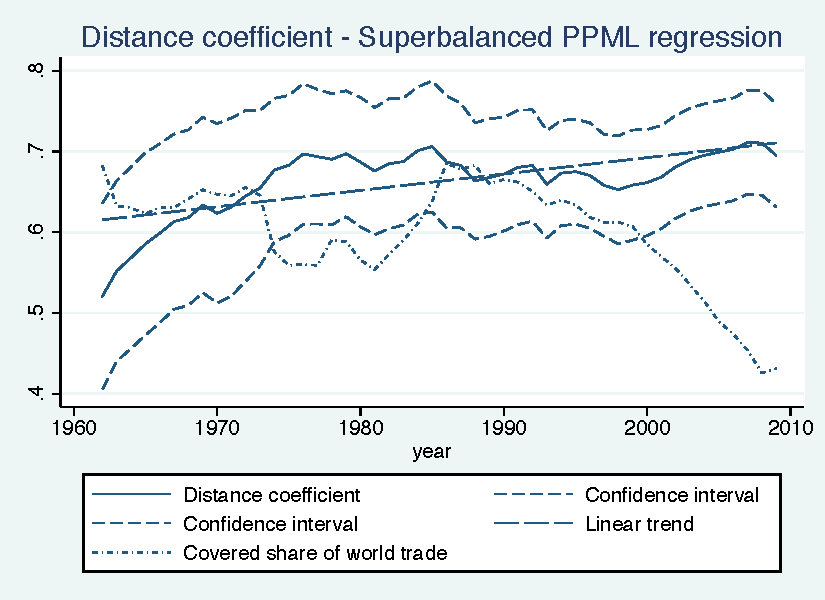
\includegraphics[trim = 0mm 0mm 0mm 9.5mm, clip,height=2.5in]{graph4.pdf}}
\end{center}
\end{figure}
\end{frame}
\fi
%say: I only show composition and FTA results
\begin{frame}[plain]\frametitle{FTAs(1)}
\begin{figure}[h!]
%\caption{Distance coefficient controlling for FTAs (full sample) \label{fig:ftas}}
\begin{center}
\setlength{\fboxrule}{1pt} %makes border lines thick
\setlength{\fboxsep}{.1in} %increases distance to border
\fbox{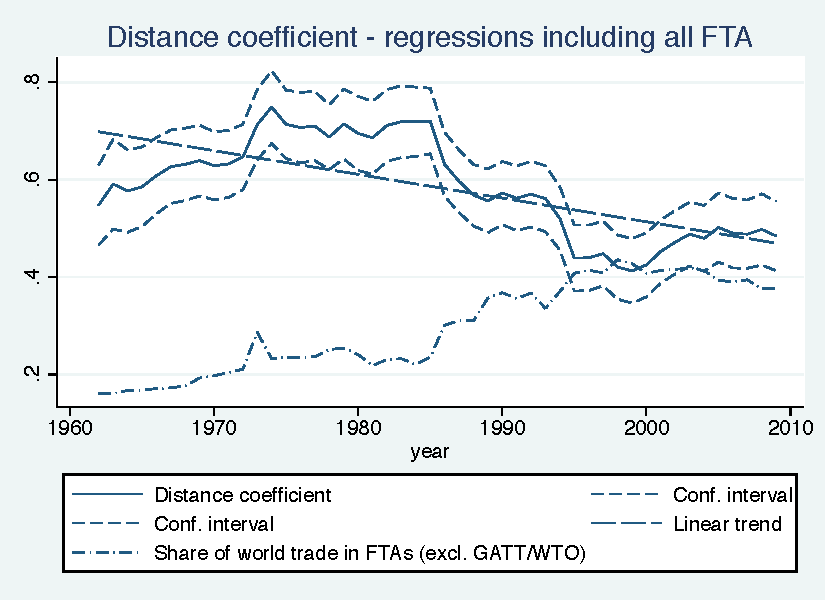
\includegraphics[trim = 0mm 0mm 0mm 9.5mm, clip,height=2.5in]{graph6.pdf}}
\end{center}
\end{figure}
\end{frame}

\begin{frame}[plain]\frametitle{FTAs(2)}
\begin{figure}[h!]
\caption{Share of intra-FTA trade among nearby countries (2000km or less)
\label{fig:ftascontig}}
\begin{center}
\setlength{\fboxrule}{1pt} %makes border lines thick
\setlength{\fboxsep}{.1in} %increases distance to border
\fbox{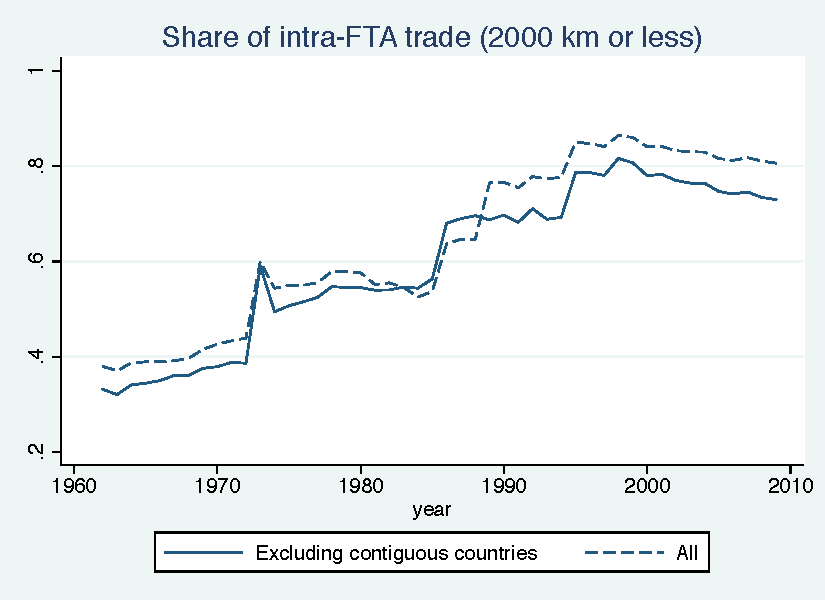
\includegraphics[trim = 0mm 0mm 0mm 9.5mm, clip,height=2.5in]{fta_proximity.pdf}}
\end{center}
\end{figure}
\end{frame}

\begin{frame}[plain]\frametitle{Summary (PPML)}
\begin{table}[H]
%\caption{Evolution of the distance coefficient depending on sample, composition, FTA effects \label{tab:summary1}}
\begin{center}
\begin{tabular}{|l|p{1in}|p{1in}|}
\hline
           & {\bf \% change relatively to baseline} & {\bf Total change 1962-2009} \\
\hline
Baseline  &     &  1.07 \\
\hline
Sample effect &        7\% &    1.14 \\
\hline
Composition effect &         7\% &     1.14 \\
\hline
FTA effect &        -54\% &         0.49 \\
\hline
Composition + sample &          7\% &         1.14 \\
\hline
Composition + FTA &      -29\% &        0.75 \\
\hline
Sample + FTA &       -59\%   &       0.44 \\
\hline
Sample + Composition + FTA &     -54\% &    0.49 \\
\hline
%\multicolumn{5}{l}{\begin{footnotesize}Results reported in the last two columns correspond to a geometric trend. \end{footnotesize}}\\
\end{tabular}
\end{center}
\end{table}
\end{frame}
%share of total trade within FTAs increases from less than 20\% to more than 40\% of trade between 1962-2009 while the share of trade between countries situated closeby (less than 2000 km: first decile of distance distribution of trade) which takes place within FTAs has increased from 38 to 79\% over the same period.
\if 0
\begin{frame}[plain]\frametitle{Robustness of puzzle}
\vspace{0.3cm}
\begin{itemize}
\item Combining the three effects:
\item dominated by FTA: makes puzzle disappear
\item but explanation unsatisfactory (endogeneity; proximity controls)
\vspace{.3cm}
\item Admit growing role of distance is robust
\item what does this mean?
\end{itemize}
\end{frame}
\fi

\section{Interpreting properly the distance coefficient}
\subsection{The heterogeneity dimension in each model}
\begin{frame}\frametitle{Ingredients of the puzzle}
\begin{itemize}
\vspace{0.3cm}
\item The distance coefficient is the elasticity of trade to distance
\begin{itemize}
\item Trivial: the whole point of log-linear equations
\item Still the case in the Poisson specification
\end{itemize}
\vspace{0.3cm}
\item It is a product of two coefficients:
\begin{itemize}
\item Elasticity of trade flows to trade costs $\zeta$
\item Elasticity of trade costs to distance $\rho$
\end{itemize}
\vspace{0.3cm}
\item The `death of distance' intuition is really about the elasticity of trade costs to distance
\item Which should be going down
\item But it does not tell much about the heterogeneity dimension, i.e. the trade elasticity $\zeta$
\end{itemize}
\end{frame}

\begin{frame}[plain]\frametitle{Short incursion in microfoundations (1)}
\begin{itemize}
\item The gravity equation can be justified by three families of theories:
\vspace{0.3cm}
\item Ricardian framework 
%(Eaton and Kortum (2002))
\\ Homogeneous goods
\\ Shop around the world for lowest cost supplier (intersectoral productivity heterogeneity)
\vspace{0.3cm}
\item Heterogeneous firms framework: 
%(Melitz (2003) / Chaney (2008))
\\ Trade because all firms produce different varieties
\\ A subset of firms enters export markets (intrasectoral productivity heterogeneity)
\vspace{0.3cm}
\item Armington framework 
%(Anderson and Wincoop (2003))
\\ Trade because consumers value variety 
\\ Country-specific goods (heterogeneity: degree of substitutability between bundles)
%\vspace{0.3cm}
%\item Consequences for the elasticity of trade to trade costs?
\end{itemize}
\end{frame}
%All theoretical frameworks used to derive the gravity equation are characterized by a common feature: the elasticity of trade flows to trade costs, the `trade elasticity', is decreasing in the degree of heterogeneity observed in a single dimension, and it is this dimension which is framework-specific. In the Ricardian framework, heterogeneity is intra-country and inter-sector: it measures the degree of dispersion in production efficiency within countries across goods, with the dispersion parameter assumed common across countries and sectors. In the Armington framework, the dimension of heterogeneity is the flipside of the Ricardian framework. Heterogeneity is inter-country and intra-sector, and corresponds to the parameter which measures the degree of perceived substitutability of country-specific varieties of each good. In the monopolistic competition framework with firm heterogeneity, the dimension of heterogeneity is intra-country and intra-sector. It is captured by the parameter which measures the degree of dispersion in firm productivity within a given sector, and this parameter is assumed common to all countries.
\begin{frame}[plain]\frametitle{Short incursion in microfoundations (2)}
\vspace{.3cm}
\begin{itemize}
\item Ricardian framework: 
\begin{itemize}
\item Distance coefficient: $\rho\theta$
\item $\theta$ captures intersectoral productivity dispersion
\item if sectors have similar productivity \\ $\rightarrow$ small differences in variable costs have a large effect on trade flows
\\ $\rightarrow$ high elasticity of trade to trade costs
\end{itemize}
\vspace{.3cm}
\item Monopolistic competition between heterogeneous firms:
\begin{itemize}
%\item assume fixed costs of trade are not distance-dependent
\item Distance coefficient: $\rho\gamma$
\item $\gamma$ captures productivity dispersion across firms (parameter of Pareto)
\item if distribution decays swiftly, higher probability that productivity cut-off for exporting is close to the mass of firms \\ $\rightarrow$  small differences in variable costs have large effect on entry 
\\ $\rightarrow$ high elasticity of trade to trade costs
\end{itemize}
\end{itemize}
\end{frame}

\begin{frame}[plain]\frametitle{Short incursion in microfoundations (3)}
\begin{itemize}
\item Armington framework
\begin{itemize}
\item Distance coefficent:  $\rho(\sigma-1)$
\item $\sigma$ captures degree of similarity between country-specific product bundles
\item if the set of goods produced by different countries is similar \\ $\rightarrow$ high Armington elasticity 
\\ $\rightarrow$ high elasticity of trade to trade costs
\end{itemize}
\vspace{0.3cm}
\item In all cases: elasticity of trade flows to trade costs is inversely related to heterogeneity 
\end{itemize}
\end{frame}

\subsection{The heterogeneity dimension captured in our data}
\begin{frame}\frametitle{Measuring the trade elasticity}
\vspace{0.3cm}
\begin{itemize}
\item Features of our data: information on bilateral trade flows and unit values
\item To measure efficiency heterogeneity: need information on domestic prices 
\begin{itemize}
\item intuition: country-specific cut-off for entry common to all exporters 
\item price distribution in destination across all sources needed to estimate shape parameter of productivity distribution
\end{itemize}
\vspace{0.3cm}
\item However we can measure substitutability across frameworks
\begin{itemize}
\item use variation of market shares of country-level composite goods across export markets 
\item construct relative prices of product bundles
\item estimate the aggregate Armington elasticity in cross section
\end{itemize}
\item The estimated parameter is the trade elasticity in the Armington framework
\end{itemize}
\end{frame}
\noteLA{Say: for this parameter to be valid across frameworks means making a strong assumption on fixed costs of trade: so small that all export}
%\subsection{Consistent aggregation procedure to get relative prices}
\noteLA{Say: in Armington model, producer heterogeneity not modelled: source-specific cost component gives directly the price of the exported good: trade elasticity can be estimated using source-specific price distributions}

\begin{frame}[plain]\frametitle{Relative prices of product bundles}
\begin{itemize}
\item Consistent aggregation procedure to get relative prices
\begin{itemize}
\item CES preferences at inter- and intrasectoral level
\item Intra- and intersectoral elasticities assumed equal
\item Write sector-specific demand equation 
\item Sum across all sectors 
%\item Use approximation that for large number of sectors, log of sum approx. equal to sum of logs
%(Imbs and Mejean)
\end{itemize}
\item Gives market share equation for aggregate bilateral trade as a function of the weighted average of sectoral relative prices of exporter in destination
\begin{eqnarray}
\ln\left[\frac{X_{ij}}{Y_j}\right]&\approx&-(\sigma-1)\ln\left[\sum_{k=1}^K{\omega_{j}(k)\frac{P_{ij}(k)}{P_j(k)}}\right] \nonumber
\end{eqnarray} 
\item Exponentiating gives equation estimated in Poisson:
\begin{eqnarray}
X_{ij}/Y_{j}&=&\exp{\left[\lambda_{0}-(\sigma-1)\ln{\left(\sum_{k}\omega_k\frac{P_{ij}(k)}{P_{j}(k)}\right)}+fe_{i}+fe_{j}\right]}\eta_{ij} \nonumber
\end{eqnarray}
\end{itemize}
\end{frame}

\section{Estimation strategy and results}
\subsection{Benchmark estimation}
\begin{frame}\frametitle{Dealing with missing unit values}
\begin{itemize}
\item Trade flow observed, but information on quantities missing
\item On average, this is the case for 14\% of total trade
\vspace{0.3cm}
\item Use stepwise price imputation procedure
\begin{itemize}
\item construct relative prices at highest disaggregation level
\item construct next level relative price as weighted average of observed relative prices
\item destination-specific weights at each step
\item repeat at each aggregation level
\end{itemize}
\vspace{0.3cm}
\item assumption: missing unit values can be best approximated by observed prices for similar goods
\end{itemize}
\end{frame}

\begin{frame}[plain]\frametitle{Dealing with zero trade flows}
\begin{itemize}
\item Under model assumptions some trade would be observed in every sector between each pair
\item Zero trade flows prevalent: from 86-90\% of possible observations at 4-digit level
\item Assumption: statistical, not structural zeros linked to data collection thresholds
\item Same stepwise procedure used for price imputation
\item Corresponds to assumption that unobserved relative price equal to observed
\item Problem: unobserved prices much higher than imputed prices
%weighted average across goods
\end{itemize}
\end{frame}

\begin{frame}[plain]\frametitle{Proportion of zero trade flows as a function of market share}
\begin{table}[H]
%\caption {\textbf{Proportion of zero trade flows as a function of market share} \label{tab:ztf1pois}} 
\begin{tabular}{lccc}
%\hline
%\multicolumn{3}{l}{\textbf{depvar:}} \\
\multicolumn{3}{l}{Share of ZTF \if 0 (Destination fixed effects included)\fi } \\
%\hline
% &  & (1) & (2) \\
\hline
 &  &  & \\
 & ms & -0.0427\textbf{***} & -0.2573\textbf{***} \\
 &  &  (0.0001) & (0.013) \\
\vspace{2pt} \\
 & year & -0.0033\textbf{***} & -0.0024\textbf{***} \\
 &  &  (0.0000) & (0.000) \\
\vspace{2pt} \\
 & $ms*year$ & & 0.0001\textbf{***} \\
 &   &  & (0.000) \\
\vspace{2pt} \\
 & constant & 6.0976\textbf{***} & 4.2515\textbf{***} \\
 &  & (0.0366) & (0.134) \\
 &  &  &\\
\hline
 & Observations & 657001 & 657001 \\ 
%\hline
%\vspace{2pt} \\
%\multicolumn{7}{l}{\begin{footnotesize}Notes: The share of ZTF is computed at the SITC 4-digit level. The estimation is conducted in PPML\end{footnotesize}} \\
%\multicolumn{7}{l}{\begin{footnotesize}in order to include observations where ztf=0. The log of the market share is used in the estimation.\end{footnotesize}} \\ 
%\multicolumn{7}{l}{\begin{footnotesize}Destination fixed effects are included in (3) and (4). Robust standard errors are in parentheses. *** p$<$0.01.\end{footnotesize}} \\
\end{tabular}
\end{table}
\end{frame}

\begin{frame}[plain]\frametitle{Overestimation bias}
\begin{itemize}
\item Underestimation factor not constant across exporters 
\begin{itemize}
\item share of ztf decreasing in market share
\item reduction in share of ztf proceeds at quicker pace for small exporters
%coefficient for the interaction term for the market share and year is significant and positive
\end{itemize}
\item Relative price underestimated by more for small exporters
\item For given distribution of market shares, true underlying distribution of prices is greater than observed distribution
\item Estimated parameter overestimates the true substitutability parameter
\item But less so overtime
\item If estimated elasticity increases, this is a lower bound on true parameter evolution
\end{itemize}
\end{frame}
%Table \ref{tab:zdesc4} presents the predicted share of ztf for four types of exporters in 1962 and 2009. For a very small exporter with .02\% market share, the initial share of ztf is predicted to be .95, and it is reduced to .83 by 2009, i.e. a 12 percentage point decrease. Consider a relatively big exporter, with a 10\% market share: its share of ztf is reduced from .72 to .65, a 7 percentage point decrease. As the gap between the share of ztf for big and small exporters is reduced overtime, the overestimation bias of $\widetilde{\sigma}$ is progressively reduced.
\if 0
\begin{frame}[plain]\frametitle{Results}
\begin{figure}[h!]
\begin{center}
\setlength{\fboxrule}{1pt} %makes border lines thick
\setlength{\fboxsep}{.1in} %increases distance to border
\fbox{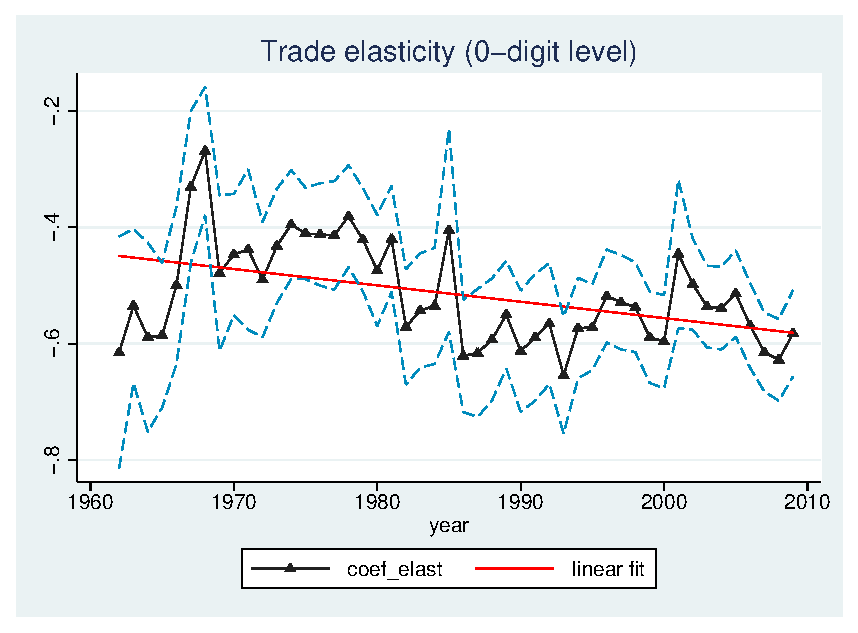
\includegraphics[trim = 0mm 0mm 0mm 9.5mm,clip,height=2.6in]{elast_real_0digit.eps}}
\end{center}
\caption{Estimated $(1-\widetilde{\sigma})$ \if 0 {, stepwise construction of the relative price} \fi \label{fig:elastreal0}}
\end{figure}
\end{frame}
\fi
%Figure \ref{fig:elastreal0} presents the results on the evolution of $(1-\widetilde{\sigma})$ obtained when (\ref{eqn:15}) is estimated on annual crossections of the COMTRADE dataset. The absolute value of trade elasticity has increased by 33\% from 1962 to 2009. This corresponds to an annual increase of .6\% per year.\footnote{The coefficient of the geometric fit is significant at 1\% level.} 
\begin{frame}[plain]\frametitle{Results}
\begin{figure}[h!]
\begin{center}
\setlength{\fboxrule}{1pt} %makes border lines thick
\setlength{\fboxsep}{.1in} %increases distance to border
%\fbox{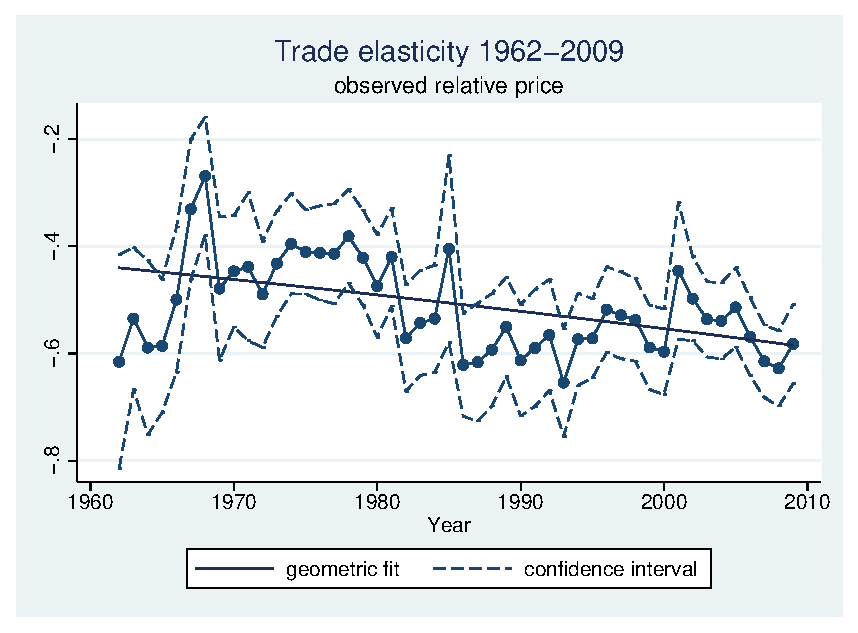
\includegraphics[0 trim = 0mm 0mm 0mm 9.5mm,clip,height=2.6in]{elast_bench.eps}}
\fbox{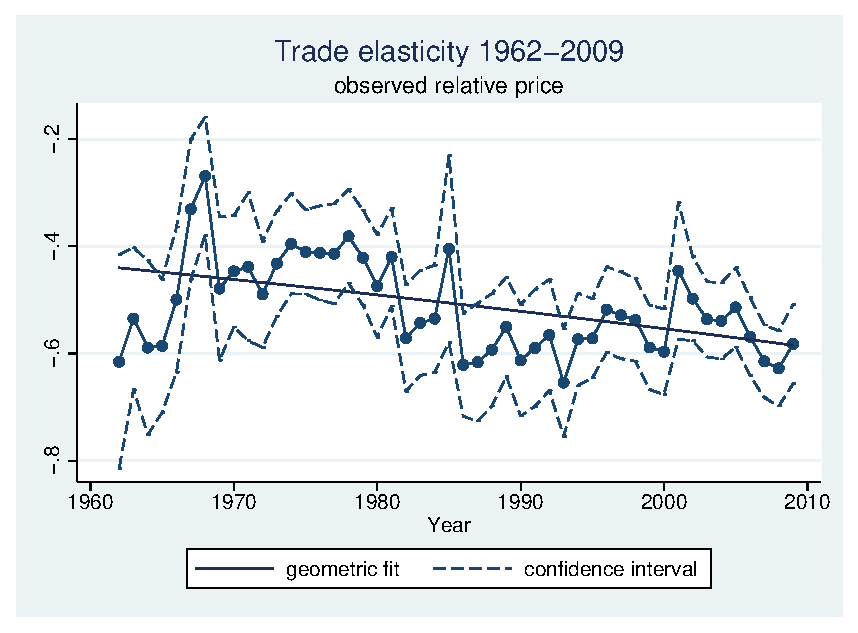
\includegraphics[height=2.5in]{elast_bench.eps}}
\end{center}
%\caption{Estimated $(1-\widetilde{\sigma})$ \label{fig:elastreal0}}
\end{figure}
\begin{itemize}
\item 33\% increase in parameter 1962-2009
\item corresponds to annual increase of .6\% per year 
\end{itemize}
\end{frame}

\subsection{Robustness checks}
\begin{frame}[plain]\frametitle{Changing the dataset: BACI}
\begin{figure}[h!]
\begin{center}
\setlength{\fboxrule}{1pt} %makes border lines thick
\setlength{\fboxsep}{.1in} %increases distance to border
\fbox{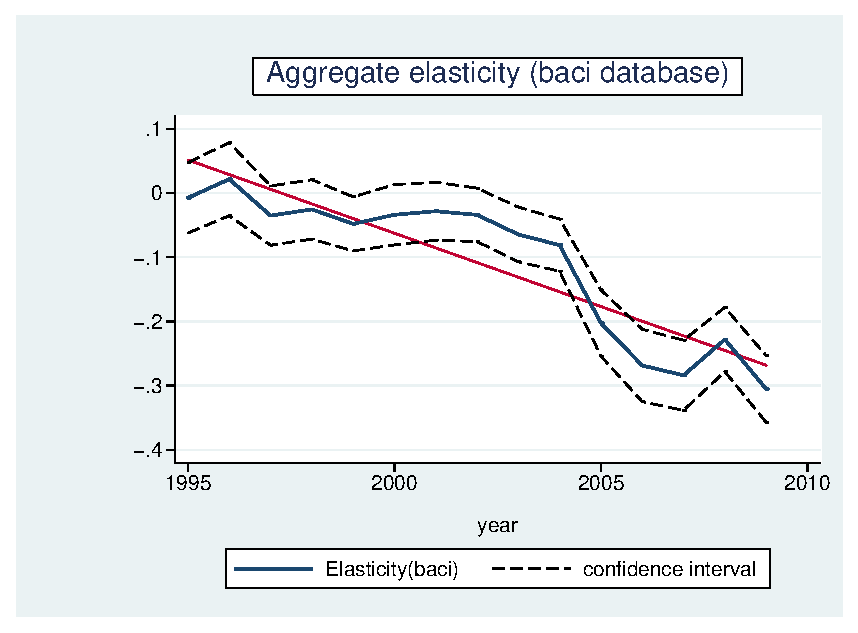
\includegraphics[height=2.5in]{elast_baci_1995_2009.eps}}
\end{center}
\caption{Estimated $(1-\widetilde{\sigma})$, BACI database \label{fig:baci}}
\end{figure}
\end{frame}
%why baci? HS-1992 6-digit disaggregation level for 1995-2009; improved quality of relative prices of product bundles: reduced number of missing unit values (1-3\% total trade); stable share of ztf

\begin{frame}[plain]\frametitle{Instrumenting: motivation}
\vspace{0.3cm}
\begin{itemize}
\item Results subject to caution?
\begin{itemize}
\item attenuation bias (if supply schedules not horizontal) 
\item matters not only for level, but for evolution (Feenstra(1994))
%estimated coefficient suffers from attenuation bias due to not controlling for potentially positive and finite supply elasticities
\end{itemize}
\vspace{0.3cm}
\item Objective: capture exporter-specific shocks to the price of the composite good which are not demand-driven
%such as exogenous shocks to the price of inputs
\vspace{0.3cm}
\item Indicator: GDP price level (Penn World Tables: 189 countries, 1950-2009)
\end{itemize}
\end{frame}

\begin{frame}[plain]\frametitle{Instrumenting: procedure}
\vspace{0.3cm}
\begin{itemize}
\item compute relative prices for exporter-specific composite goods 
%in each destination 
\item compute evolution of GDP price levels of trading partners, weighted by market shares (common currency)
%this amounts to computing the evolution of the relevant real exchange rate for each specific bilateral trade relation.
\item compute hypothetical relative price in $t$ for each exporter as:
\begin{itemize}
\item product of its relative price in $(t-s)$
\item evolution of its GDP price level between $t$ and $(t-s)$ relatively to all other partners
\end{itemize}
\item predict relative price of each exporter in $t$: regress observed relative price on hypothetical relative price.
\item Idea: get an instrumented relative price which depends on past relative price and relative evolution of GDP price level.
\item Estimate market share equation using instrumented relative prices
%s is number of lags
\end{itemize}
\end{frame}

\begin{frame}[plain]\frametitle{Instrumenting: one lag}
\begin{figure}[h!]
\begin{center}
\setlength{\fboxrule}{1pt} %makes border lines thick
\setlength{\fboxsep}{.1in} %increases distance to border
\fbox{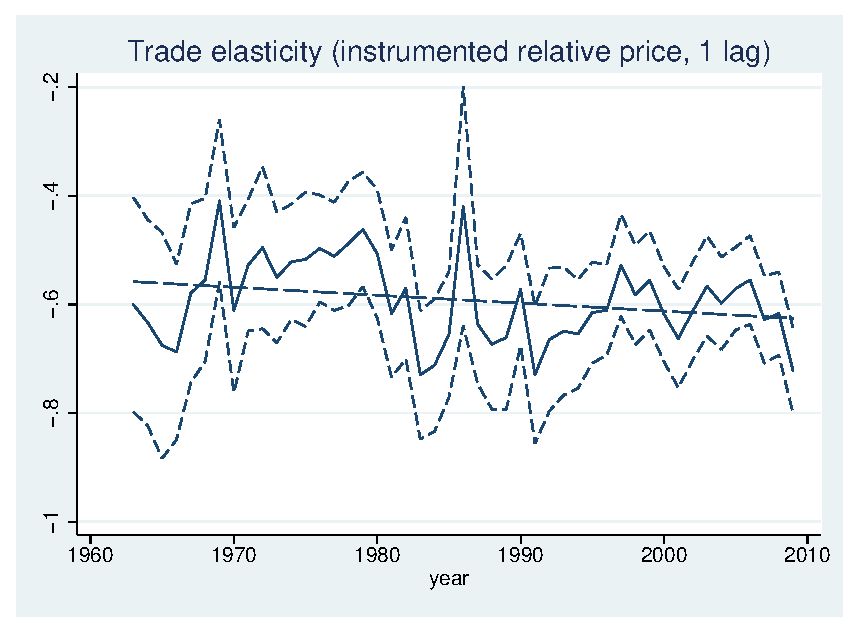
\includegraphics[height=2.5in]{elast_instr_1lag_v7.eps}}
\end{center}
%\caption{Estimated $(1-\widetilde{\sigma})$, instrumented relative price of composite good, 1 lag \label{fig:instr1}}
\end{figure}
\begin{itemize}
\item reassuring: level of parameter increases by 9\%
\item results on evolution hold: 13\% increase
\end{itemize}
\end{frame}
%It could be argued that allowing for just one lag inadequately captures the temporal relationship between shocks to inputs' prices and their pass-through to the price of exported output. Indeed, if prices are relatively persistent, the instrumenting procedure would amount to little more than replacing observed prices in $t$ with lagged observed prices in $(t-1)$. We therefore also estimate (\ref{eqn:15}) using as instrument the evolution of each exporter's GDP price level relatively to all other trading partners in the destination between $(t-s)$ and $t$ where $s=1,...,10$.

\begin{frame}[plain]\frametitle{Increasing the number of lags}
\begin{figure}[h!]
\begin{center}
\setlength{\fboxrule}{1pt} %makes border lines thick
\setlength{\fboxsep}{.1in} %increases distance to border
\fbox{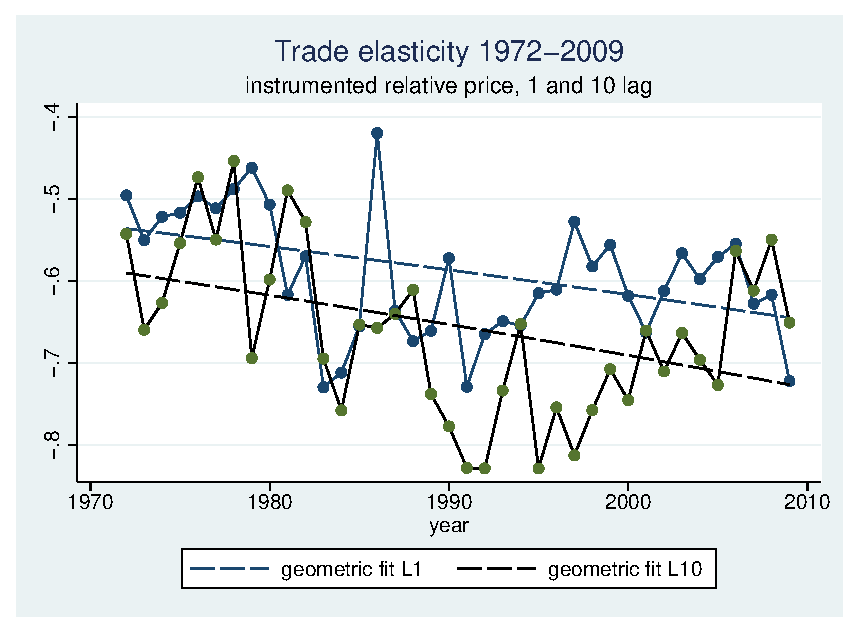
\includegraphics[height=2.5in]{elast_l1_l10.eps}}
\end{center}
%\caption{Estimated $(1-\widetilde{\sigma})$, instrumented relative price of composite good \label{fig:instr3}}
\end{figure}
\begin{itemize}
\item level increases with number of lags: 22\% for 10 lags
\item results on evolution hold: 23\% increase in 1972-2009 
%(20\% for 1 lag)
\end{itemize}
\end{frame}
%say: level becomes more stable as we increase nb of lags, and level increases; slope preserved

\if 0
\begin{frame}[plain]\frametitle{Increasing the number of lags}
\begin{figure}[h!]
\begin{center}
\setlength{\fboxrule}{1pt} %makes border lines thick
\setlength{\fboxsep}{.1in} %increases distance to border
\fbox{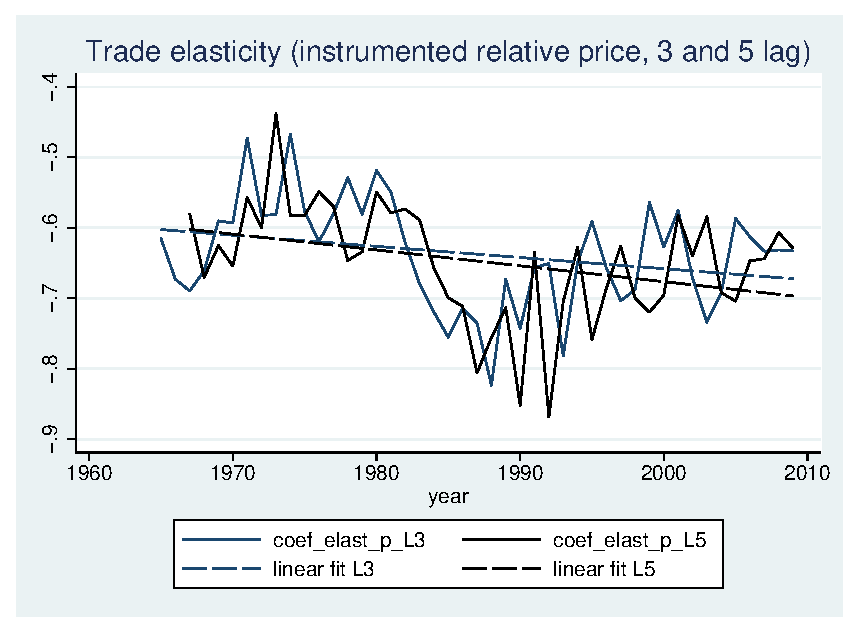
\includegraphics[height=2.5in]{elast_instr_3_5lag_v7.eps}}
\end{center}
%\caption{Estimated $(1-\widetilde{\sigma})$, instrumented relative price of composite good \label{fig:instr2}}
\end{figure}
\begin{itemize}
\item level increases with number of lags: 20\% for 5 lags
\item results on evolution hold: 18\% increase in 1967-2009
\end{itemize}
\end{frame}
\fi

\section{Conclusion}
\begin{frame}\frametitle{Is there a distance puzzle left?}
\begin{itemize}
\item empirical evidence on 13\% increase in substitutability parameter
\item this is aggregate trade elasticity in Armington framework
\item combining with 7\% increase in distance elasticity
\item provides a direct explanation of the distance puzzle
\item economic interpretation of increased perceived substitutability of product bundles?
\begin{itemize}
\item increasing similarity in set of traded goods across countries
\item composition effects (changes in range or shares of traded goods)
\end{itemize}
\item Not done: separate out net effect of increased perceived similarity
\item Not feasible? parameter estimated on aggregate data is not a weighted average of sectoral parameters
\end{itemize}
\end{frame}

\end{document}